\section*{Results and Discussion}

\graphicspath{{../Rscript/CMG_Rscript_files/figure-gfm/}}

\subsection*{Description of the set of bins}

Information about the sequences used for this project were retrieved from the \textit{metadata} and the \textit{bin data} files that were provided with the data. \textit{Metadata} provides an insight about the experiments from which our MAGs were obtained. This includes data about the hosts from whom the samples were taken: their health conditions, age, gender, and country, as well as information about the sequences: number and length of the reads, number of bases and other information concerning the experiments. The two reference genomes are curated by the NCBI and are not reported in this file, and for the other datasets not all the features are always provided. The \textit{bin data} file reports completeness and redundancy of the MAGs, including the reference genomes.\\

The set of MAGs come from 9 different datasets, all of them working on stool samples. For what concerns the patients involved, three main study conditions can be identified: colorectal cancer (CRC), adenoma and control. The control group is the most numerous group, composed by 19 samples. The CRC and the adenoma groups present respectively 7 and 3 samples. Patients in the control group are cancer-free but not all of them are healthy: 7 of them suffer from fatty liver, hypertension, type two diabetes or a combination of the three. Moreover, all cancer patients are reported to be associated with one or more of these diseases (Fig. \ref{fig:studyConditions} (A)). All hosts are aged 35 or older, in particular 9 of them are considered senior (older than 65 years old). The samples are almost equally distributed between female and male patients (12 females and 13 males). The hosts come from 8 different countries, all of them from Europe with Austria being the most represented nation (18 samples), except for one patient from Argentina and one from Guinea. Only one sample was obtained from a non-westernized host and its country of origin is Argentina (Fig \ref{fig:studyConditions} (B-E)). All the analyzed MAGs were obtained from sequencing experiments carried out with the IlluminaHiSeq technology and the minimum read length indicated for each dataset shows that quality control was performed and only high-quality reads longer than 30 nucleotides were retained.\\

\begin{figure}[!h]
    \centering
    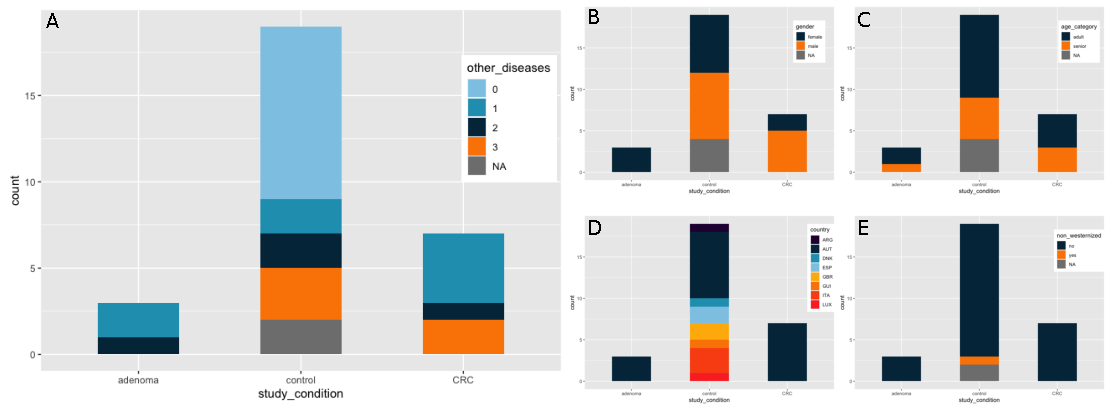
\includegraphics[width=\textwidth]{study_conditions.pdf}
    \caption{\textbf{Study conditions.} Number of samples per study condition (CRC, adenoma, control). Distribution of: A) other diseases, B) gender, C) age, D) country of origin and E) westernized/non westernized in each study condition group.}
    \label{fig:studyConditions}
\end{figure}

Completeness is the estimate of how completely a MAG represents a full genome based on the presence or absence of single-copy core genes, which are the genes found in the vast majority of genomes. Redundancy is the measure of how many single-copy core genes are found within a genome\cite{anvio}. All MAGs analyzed have high completeness that spans from 90.33\% to 100\%. In addition to the reference genomes, there are 2 other datasets presenting 100\% completeness. Moreover, all MAGs present low redundancy, from 0 to 4.48\%, with 5 of them having zero redundancy reported (Fig. \ref{fig:completeness}). These values indicate that each sequence has high quality and has been rightfully considered as a MAG. Redundancy can be interpreted as an indication for the presence of contamination, because high redundancy levels could mean that more than one population of bacteria were considered in the assembling of the genome. Despite the good redundancy values reported, it is not wise to completely exclude the possibility of contamination since redundancy is not the sole indicator of contamination.

\begin{figure}[!h]
    \centering
    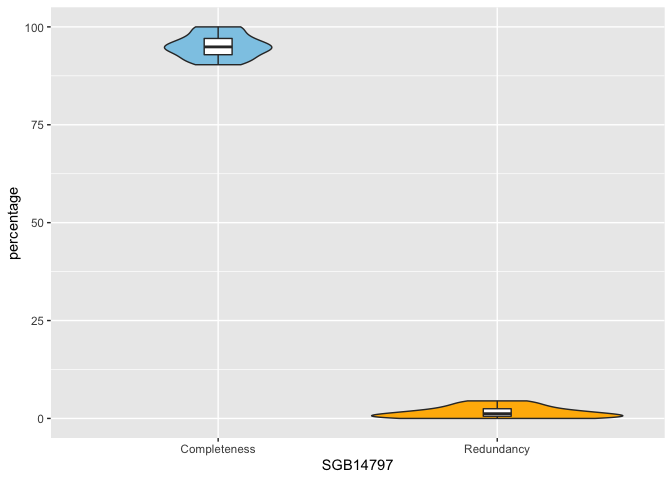
\includegraphics[width=0.5\textwidth]{completeness_redundancy-1.png}
    \caption{\textbf{Completeness and redundancy.} The violin plot shows how the percentages of completeness and redundancy are distributed among the set of MAGs. There are no genomes with completeness below 90\% and no genomes with redundancy above 5\%}
    \label{fig:completeness}
\end{figure}

\subsubsection*{Taxonomic assignment}

The results of the \textit{PhyloPhlAn} analysis conducted on all the MAGs considered for this project are reported in the table \ref{tab:taxonomy}. The first analysis gave as result two MAGs assigned to a diffeerent Phylum (\textit{Firmicutes}) with respect to all the others. These datasets were discarded from the project, since they were two low-quality incomplete genomes. Afterwards, the \textit{PhyloPhlAn} output resulted consistent for each putative genome, confirming that they are all correctly clustered in the same species-level genome bin (SGB). The species of this SGB is \textit{Adlercreutzia equolifaciens}.\\

\begin{table}[h]
\centering
\begin{tabular}{|c|c|}
    \hline
    \textbf{Kingdom} & Bacteria \\
    \hline
    \textbf{Phylum} & Actinobacteria \\
    \hline
    \textbf{Class} & Coriobacteria \\
    \hline
    \textbf{Order} & Eggerthellales \\
    \hline
    \textbf{Family} & Eggerthellaceae \\
    \hline
    \textbf{Genus} & Adlercreutzia \\
    \hline
    \textbf{Species} & equolifaciens \\
    \hline
\end{tabular}
\caption{Taxonomic assignment of the set of MAGs}
\label{tab:taxonomy}
\end{table}

\textit{Adlercreutzia equolifaciens} are Gram positive, obligately anaerobic coccobacilli that can be found in human feces. They are capable of metabolizing equol from daidzein, a type of isoflavone found in soybeans and other similar plants\cite{Adlercreutzia}. Equol is a nonsteroidal estrogen produced by the gut microbiota of 30-50\% of the human population. Some evidence suggests that it might play an important role in lipid metabolism\cite{equol}.